\documentclass{article}
\usepackage[utf8]{inputenc}
\usepackage{lipsum}
\usepackage{setspace}
\usepackage{geometry}
\usepackage{graphicx} %pt includere img
\usepackage{caption} %pt captions la imagini
\usepackage{subcaption} 
\usepackage{float} %pozitionare poze
\usepackage{hyperref}  %pt url
\geometry{a4paper, margin=1in}

\title{Ribosomes: Structure, Function and Importance}
\author{Mara-Andreea Spataru \\ Grupa 341}
\date{\today}

\begin{document}
	
	\maketitle
	
	\section*{Introduction}
	In order to get to what ribosomes represent, we must first describe or define what the cell is, then we must understand the difference between eukaryote and prokaryote cells, so we can finally state what exactly are the ribosomes, their role, and different interesting aspects about them.
	
	\section*{Cell Structure}
	Living organisms have two types of organization: prokaryote organization and eukaryote organization, each having its own structure and chemical composition.
	
	\begin{figure}[h]
		\flushleft  %aliniere la stg
		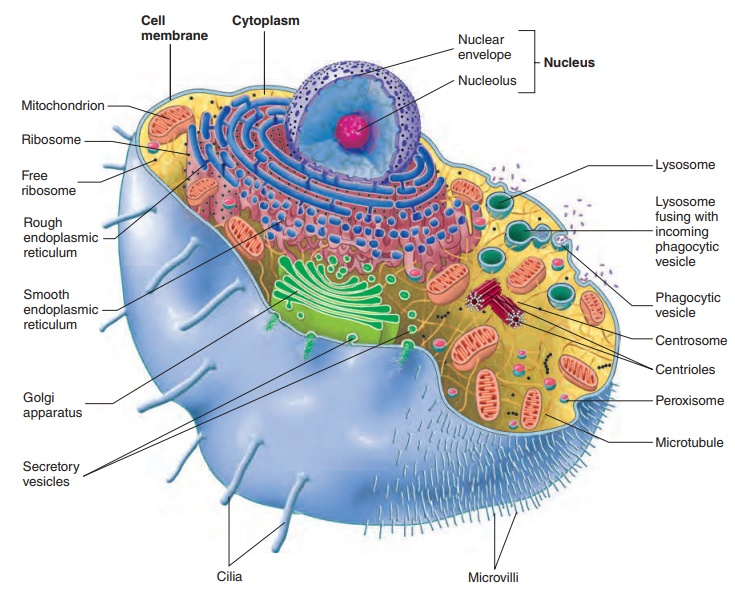
\includegraphics[width=0.6\textwidth]{C:/Users/maras/OneDrive/Desktop/an 3/Bioinformatica/Tema2 ribozomi/cellstructure.jpg}
		\caption{Cell structure showing various organelles. Source: \url{https://www.brainkart.com/article/Cell-Structure_21751/}}
	\end{figure}
	
	The prokaryotic structure (characteristic for bacteria and blue-green algae) is a simple structure. Prokaryotic cells do not contain their genetic material in a nucleus, so they are a type of cell that does not have a nucleus.
	
	The eukaryotic structure is more complicated, and it is characteristic to other forms of algae, fungi, and the entire animal kingdom.
	
	\begin{figure}[h]
		\centering  %centrare pt intregul block
		\begin{subfigure}{0.42\textwidth}
			\centering
			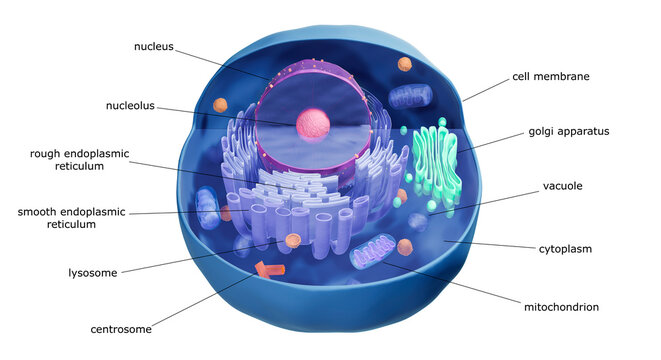
\includegraphics[height=5cm]{C:/Users/maras/OneDrive/Desktop/an 3/Bioinformatica/Tema2 ribozomi/eukaryoticcell.jpg}
			\caption{Eukaryotic cell diagram. Source: Adobe Stock Images (\url{https://stock.adobe.com/search?k=eukaryotic+cell})}
		\end{subfigure}
		\hfill  %creare spatiu orizontal intre img
		\begin{subfigure}{0.42\textwidth}
			\centering
			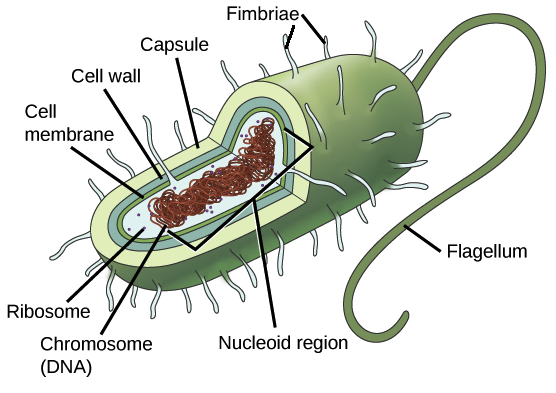
\includegraphics[height=5cm]{C:/Users/maras/OneDrive/Desktop/an 3/Bioinformatica/Tema2 ribozomi/prokaryoticcell.jpg}
			\caption{Prokaryotic cell. Image credit: modified from "Prokaryotic cells: Figure 1" by OpenStax College, Biology, CC BY 3.0. Source: \url{https://www.khanacademy.org/science/biology/structure-of-a-cell/prokaryotic-and-eukaryotic-cells/a/prokaryotic-cells}}
		\end{subfigure}
	\end{figure}
	
	The cell is the elementary, morphologic and functional unit of all living organisms. The cell is made up of three parts: the nucleus, which contains the genetic material known as DNA; the cytoplasm, which is the watery environment in which most biochemical activities take place; and other organelles. All of these structures perform specific and essential functions, and their integrated cooperation ensures the life and normal functioning of the cell.
	
	\section*{Ribosome Structure}
	They are divided into two separate subunits: the big one and the small one. The two are connected when synthesis takes place and then split when it is completed. Ribosomes can be found either free in the cytoplasm, where they synthesise proteins for intercellular use, or attached to endoplasmic reticulum membranes, forming the rough endoplasmic reticulum, where they synthesise proteins for secretion or membrane incorporation.
	
	\section*{Ribosome Function}
	Ribosomes are the cell's protein producers. They convert the genetic information contained in messenger RNA (mRNA) into proteins. This occurs in three phases: initiation (when the ribosome attaches to the mRNA), elongation (amino acid chain grows), and termination (synthesis is completed). During the process, the ribosome reads triplets of nucleotides and appends the matching amino acids given by the genetic code. The ribosomes have the unique role of forming peptide bonds between amino acids, hence generating the protein structure.
	
	\section*{Interesting Aspects}
	The ribosomes of the prokaryote cells are built differently from those of the eukaryotes, and this is exploited by particular antibiotics like the streptomycin because it selectively destroys bacterial ribosomes. The malfunction of the ribosome is closely linked with genetic disease, which proves that they play a vital part in maintaining the normal condition of the organism.
	
	\section*{Conclusion}
	Finally, the ribosomes are cell components essential to life because they are the ones responsible for carrying out the simple function of protein synthesis. The functional variety of living forms would not be possible without these little molecular factories, highlighting how complicated and amazing the machinery that sustains life is.
	
\end{document}	